\documentclass[a4paper,14pt]{extarticle}

\usepackage[a4paper,top=20mm,bottom=20mm,left=30mm,right=10mm]{geometry}
\usepackage[T1,T2A]{fontenc}
\usepackage[utf8]{inputenc}
\usepackage[russian]{babel}
\usepackage{indentfirst}
\usepackage{titlesec}
\usepackage{graphicx}
\usepackage{verbatim}
\usepackage{fancyvrb}

\renewcommand{\baselinestretch}{1.3}
\titleformat{\section}{\normalsize\bfseries}{\thesection}{1em}{}
\titleformat{\subsection}{\normalsize\bfseries}{\thesection}{1em}{}
\setlength{\parindent}{12.5mm}

\begin{document}

  \newpage\thispagestyle{empty}
  \begin{center}
    \MakeUppercase{
      Министерство науки и высшего образования Российской Федерации\\
      Федеральное государственное бюджетное образовательное учреждение высшего образования\\
      <<Вятский Государственный Университет>>\\
    }
    Институт математики и информационных систем\\
    Факультет автоматики и вычислительной техники\\
    Кафедра электронных вычислительных машин
  \end{center}
  \vfill

  \begin{center}
    Отчет по лабораторной работе №3\\
    по дисциплине\\
    <<Управление данными>>\\
    <<Пользовательские функции>>\\
  \end{center}
  \vfill

  \noindent
  \begin{tabular}{ll}
    Выполнил студент гр. ИВТб-2301-05-00 \hspace{5mm} &
    \rule[-1mm]{25mm}{0.10mm}\,/Макаров С.А./\\
    
    Преподаватель & \rule[-1mm]{25mm}{0.10mm}\,/Клюкин В.Л./\\
  \end{tabular}

  \vfill
  \begin{center}
    Киров 2025
  \end{center}

  \newpage
  \section*{Цель}
  Цель лабораторной работы: познакомиться с созданием пользовательских функций и триггеров в PostgreSQL, освоить работу с составными типами данных и массивами, изучить основы работы с процедурным языком PL/pgSQL.

  \section*{Задание}
  \begin{enumerate}
    \item Для любой таблицы создать функцию save имя таблицы, которая принимает на вход параметры, соответствующие её столбцам, и, если переданное значение первичного ключа равно null, выполняет запрос insert, иначе – запрос update для соответствующей строки. Функция должна вернуть значение первичного ключа вставленной или изменённой строки.
    \item Для любой таблицы, на которую имеются внешние ключи, создать функцию delete имя таблицы, принимающую на вход значение первичного ключа строки и ничего не возвращающую. Если на удаляемую строку существуют ссылки, то функция должна поднимать ошибку «Невозможно выполнить удаление, так как есть внешние ссылки».
    \item  Для таблицы, содержащей столбец с числовыми значениям, создать функцию, которая принимает на вход число – минимальное значение – и возвращает setof имя таблицы – множество строк, в которых значение числа больше или равно переданному аргументу. 
    \item Создать составной тип, содержащий не менее 2-3 полей, по крайней мере одно из которых должно быть числовым. Создать функцию, которая принимает массив объектов этого типа и минимальное значение для указанного поля. Функция должна возвращать массив отфильтрованных по переданному значению объектов.
    \item  Для любой таблицы создать таблицу log имя таблицы, которая будет содержать лог изменений по любому выбранному столбцу этой таблицы. Для этого нужны столбцы:
      \begin{itemize}
        \item[--] первичный ключ;
        \item[--] внешний ключ на выбранную таблицу;
        \item[--] дата изменения строки;
        \item[--] старое значение столбца;
        \item[--] новое значение столбца.
      \end{itemize}
      Реализовать заполнение таблицы с логом с помощью триггеров на вставку/изменение строк.
    \item Реализовать любую функцию на свой выбор, использующую для получения результата динамически формируемый запрос.
  \end{enumerate}

  \pagebreak
  \section*{Решение}
  \subsection*{Задание 1}

  Если в параметре ID дисциплины указан NULL, то функция должна создать новую запись в таблице, если указан – обновить существующую запись. В случае если мы обновим запись с ID, не существующем на данный момент в таблице, ничего не произойдет.

  Функция будет возвращать значение id строки, с которой была произведена работа.

  Далее представлен код разработанной функции:

  \noindent
  \begin{Verbatim}[tabsize=4,fontsize=\small]
CREATE OR REPLACE FUNCTION save_category (
    _id BIGINT,
    _title VARCHAR(256)
)
RETURNS BIGINT
AS $$
DECLARE
    category_id BIGINT;

BEGIN
    IF _id IS NULL THEN
        INSERT INTO categories (title)
        VALUES (_title)
        RETURNING id INTO category_id;
    ELSE
        UPDATE categories SET
            title = _title
        WHERE id = _id;

        category_id := _id;
    END IF;

    RETURN category_id;
END;
$$ LANGUAGE plpgsql;
  \end{Verbatim}

  Проверим работу функции. Для начала, посмотрим, как выглядит таблица до изменения (Рисунок 1):

  \begin{figure}[h]
    \centering
    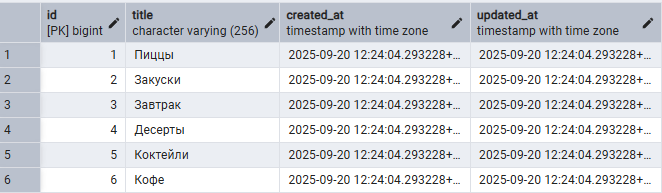
\includegraphics[width=1\linewidth]{img/t-1-1}
  \end{figure}
  \begin{center}
    Рисунок 1 – Таблица categories до изменений
  \end{center}

  Теперь выполним запрос:

  \noindent
  \begin{Verbatim}[tabsize=4,fontsize=\small]
SELECT save_category(null, 'Обед');
  \end{Verbatim}

  На рисунке 2 представлен вывод Id новой строки:

  \begin{figure}[h]
    \centering
    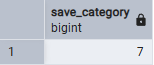
\includegraphics[width=0.2\linewidth]{img/t-1-2}
  \end{figure}
  \begin{center}
    Рисунок 2 – Id новой строки
  \end{center}

  Затем выполним запрос:

  \noindent
  \begin{Verbatim}[tabsize=4,fontsize=\small]
SELECT save_category(4, 'Сладости');
  \end{Verbatim}

  На рисунке 3 представлен вывод Id измененной строки:

  \begin{figure}[h]
    \centering
    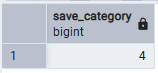
\includegraphics[width=0.2\linewidth]{img/t-1-3}
  \end{figure}
  \begin{center}
    Рисунок 3 – Id измененной строки
  \end{center}

  Проверим таблицу (Рисунок 4). Создана строка с индексом 7, а содержимое строки с индексом 4 изменено.

  \pagebreak
  \begin{figure}[h]
    \centering
    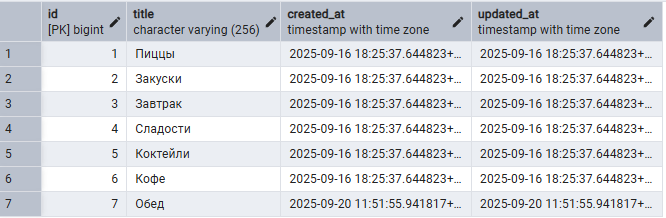
\includegraphics[width=1\linewidth]{img/t-1-4}
  \end{figure}
  \begin{center}
    Рисунок 4 – Таблица categories после изменений
  \end{center}

  \subsection*{Задание 2}
  Функция delete category будет на вход принимать ID строки, которую нужно будет удалить из таблицы.

  Если такого ID нет в таблице, то ничего не произойдет, скрипт отработает без ошибок.

  Если в других таблицах строки ссылаются на удаляемую нами строку, мы должны выдать ошибку с текстом: «Невозможно выполнить удаление, так как есть внешние ссылки.».

  Далее представлен код разработанной функции:

  \noindent
  \begin{Verbatim}[tabsize=4,fontsize=\small]
CREATE OR REPLACE FUNCTION delete_category (
    _id BIGINT
)
RETURNS VOID
AS $$
BEGIN
    DELETE FROM categories
    WHERE id = _id;

EXCEPTION
    WHEN foreign_key_violation THEN
        RAISE EXCEPTION 'Невозможно выполнить удаление,
            так как есть внешние ссылки.';
END;
$$ LANGUAGE plpgsql;
  \end{Verbatim}

  Далее нужно подготовить таблицы к тестам. Таблица до изменений представлена на рисунке 5:

  \begin{figure}[h]
    \centering
    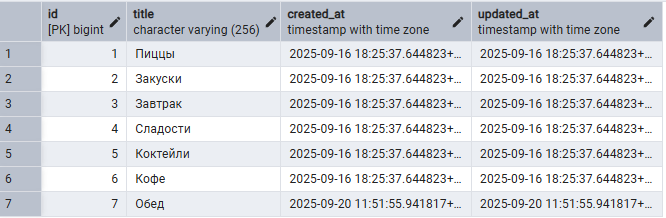
\includegraphics[width=1\linewidth]{img/t-1-4}
  \end{figure}
  \begin{center}
    Рисунок 5 – Таблица categories до изменений
  \end{center}

  Затем вызовем функцию с Id строки, на которую нет внешних ссылок. В данном примере это строка с Id 7:

  \noindent
  \begin{Verbatim}[tabsize=4,fontsize=\small]
SELECT delete_category(7);
  \end{Verbatim}

  Функция отработала успешно. Теперь вызовем функцию с Id 1:

  \noindent
  \begin{Verbatim}[tabsize=4,fontsize=\small]
SELECT delete_category(1);
  \end{Verbatim}

  Функция была завершена с ошибкой, текст которой мы указали ранее. Результат работы функции представлен на рисунке 6:

  \begin{figure}[h]
    \centering
    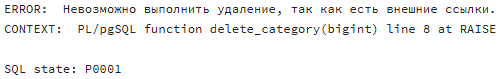
\includegraphics[width=0.8\linewidth]{img/t-2-1}
  \end{figure}
  \begin{center}
    Рисунок 6 – Результат работы функции delete category(1)
  \end{center}

  На рисунке 7 представлена функция таблицы после изменений. Строка с индексом 7 была удалена, а с индексом 1 – нет.

  \pagebreak
  \begin{figure}[h]
    \centering
    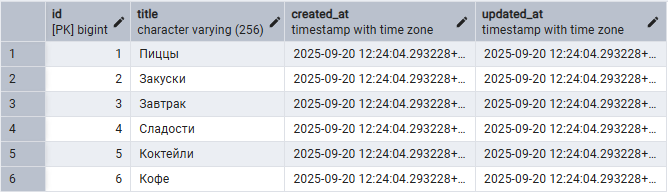
\includegraphics[width=1\linewidth]{img/t-2-2}
  \end{figure}
  \begin{center}
    Рисунок 7 – Таблица categories после изменений
  \end{center}

  \subsection*{Задание 3}
  Функция будет принимать на вход числовое значение, а затем возвращать таблицу, в которой выбранное нами значение будет больше либо равно заданного нами числового значения.

  Реализация функции будет для таблицы product variants. Фильтрация будет производиться по полю price.

  Ниже представлена разработанная функция:

  \noindent
  \begin{Verbatim}[tabsize=4,fontsize=\small]
CREATE OR REPLACE FUNCTION filter_product_variant_by_price (
    min_val INT
)
RETURNS SETOF product_variants
AS $$
BEGIN
    RETURN QUERY (SELECT * FROM product_variants 
                    WHERE price >= min_val);
END;
$$ LANGUAGE plpgsql;
  \end{Verbatim}

  Для проверки работы функции выполним запрос:

  \noindent
  \begin{Verbatim}[tabsize=4,fontsize=\small]
SELECT * FROM filter_product_variant_by_price(500);
  \end{Verbatim}

  На рисунке 8 представлена таблица, возвращаемая функцией:

  \pagebreak
  \begin{figure}[h]
    \centering
    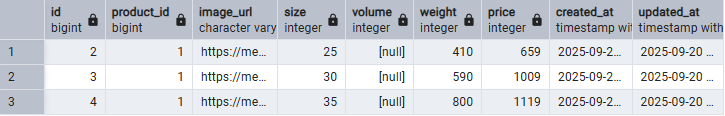
\includegraphics[width=1\linewidth]{img/t-3-1}
  \end{figure}
  \begin{center}
    Рисунок 8 – Таблица, возвращаемая функцией filter product variant by price.
  \end{center}

  \subsection*{Задание 4}
  Данная функция будет принимать на вход массив объектов составного типа данных и числовое значение, по которому будет фильтроваться массив данных и возвращаться из функции.

  Для начала необходимо создать тип данных. Составной тип данных будет называться t ingredient и содержать поля, как в таблице ingredients:

  \noindent
  \begin{Verbatim}[tabsize=4,fontsize=\small]
CREATE TYPE t_ingredient AS (
    id BIGINT,
    title VARCHAR(256),
    price INT
);
  \end{Verbatim}

  Ниже представлена разработанная функция:

  \noindent
  \begin{Verbatim}[tabsize=4,fontsize=\small]
CREATE OR REPLACE FUNCTION filter_array_of_ingredients (
    arr t_ingredient[],
    fitler_var INT
)
RETURNS t_ingredient[]
AS $$
BEGIN
    RETURN ARRAY(
        SELECT (id, title, price)::t_ingredient
        FROM ingredients
        WHERE price >= fitler_var
    );
END;
$$ LANGUAGE plpgsql;
  \end{Verbatim}

  Для проверки воспользуемся данным запросом. Он берет данные из таблицы subject, преобразует их в массив и отправляет его в качестве параметра нашей функции:

  \noindent
  \begin{Verbatim}[tabsize=4,fontsize=\small]
SELECT filter_array_of_ingredients(
    ARRAY(SELECT (id, title, price)::t_ingredient FROM ingredients),
    60
);
  \end{Verbatim}

  На рисунках 9 и 10 представлено сравнение таблицы ingredients и возврата функции filter array of ingredients:

  \begin{figure}[h]
    \centering
    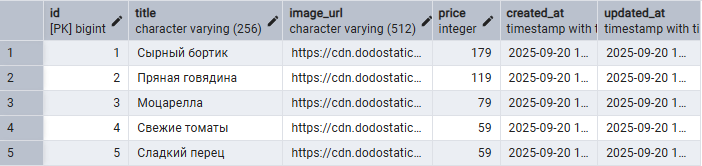
\includegraphics[width=1\linewidth]{img/t-4-1}
  \end{figure}
  \begin{center}
    Рисунок 9 – Таблица ingredients
  \end{center}

  \begin{figure}[h]
    \centering
    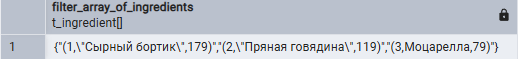
\includegraphics[width=0.8\linewidth]{img/t-4-2}
  \end{figure}
  \begin{center}
    Рисунок 10 – Вывод результата функции filter array of ingredients
  \end{center}

  Функция вернула массив объектов, отсортированных по значению 60.

  \subsection*{Задание 5}
  Данная таблица будет содержать в себе информацию о вставке/изменении таблицы ingredients:

  \begin{itemize}
    \item[--] Первичный ключ;
    \item[--] Внешнюю ссылку на строку;
    \item[--] Дату и время внесенных изменений;
    \item[--] Старое значение (если был произведен UPDATE);
    \item[--] Новое значение.
  \end{itemize}

  Ниже представлен скрипт создания таблицы:
  
  \noindent
  \begin{Verbatim}[tabsize=4,fontsize=\small]
CREATE TABLE log_ingredeints (
    id BIGSERIAL PRIMARY KEY,
    ingredient_id BIGINT,
    change_datetime TIMESTAMP WITH TIME ZONE DEFAULT CURRENT_TIMESTAMP,
    old_value INT,
    new_value INT,

    FOREIGN KEY (ingredient_id) REFERENCES ingredients(id) ON DELETE RESTRICT
)
  \end{Verbatim}

  Создадим триггерную функцию. Она будет определять, какой вид запроса был произведен, и, в соответствии с ним, корректировать запрос. Это необходимо потому, что при INSERT нам нужно заполнить поле old value значением NULL. Функция всегда будет возвращать переменную NEW.

  Ниже представлен скрипт создания функции:

  \noindent
  \begin{Verbatim}[tabsize=4,fontsize=\small]
CREATE OR REPLACE FUNCTION ingredients_trigger_func ()
RETURNS TRIGGER
AS $$
DECLARE
    old_val INT;

BEGIN
    IF (TG_OP = 'UPDATE') THEN
        old_val := OLD.price;
    ELSEIF (TG_OP = 'INSERT') THEN
        old_val := NULL;
    END IF;

    INSERT INTO log_ingredeints (ingredient_id, old_value, new_value)
    VALUES (NEW.id, old_val, NEW.price);

    RETURN NEW;
END;
$$ LANGUAGE plpgsql;
  \end{Verbatim}

  Теперь создадим триггер. Он будет срабатывать после изменений в таблице ingredients, так как нам нужно иметь записи об уже совершенных действиях. Триггер будет реагировать на запросы UPDATE и INSERT:

  \noindent
  \begin{Verbatim}[tabsize=4,fontsize=\small]
CREATE TRIGGER commit_ingredients_change
AFTER UPDATE OR INSERT
ON ingredients
FOR EACH ROW
EXECUTE PROCEDURE ingredients_trigger_func();
  \end{Verbatim}

  Чтобы проверить работу триггера, создадим новую строку в таблице ingredients, а затем изменим ее значение, подставив id новой записи:

  \noindent
  \begin{Verbatim}[tabsize=4,fontsize=\small]
INSERT INTO ingredients (title, image_url, price)
VALUES ('Острый перец халапенью', 
        'https://cdn.dodostatic.net/static
        /Img/Ingredients/11ee95b6bfdf98fb88a113db92d7b3df.png', 59);
UPDATE ingredients SET price = 89 WHERE id = 6;
  \end{Verbatim}
  На рисунке 11 можно заметить, что в таблице log ingredients добавилось 2 записи. В первой отсутствует поле old value – она соответствует добавлению нового значения. Вторая говорит нам о том, что было изменено существующее значение.

  \begin{figure}[h]
    \centering
    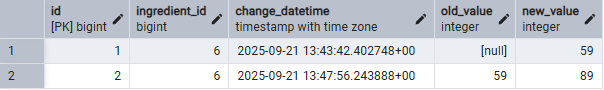
\includegraphics[width=1\linewidth]{img/t-5-1}
  \end{figure}
  \begin{center}
    Рисунок 11 – Вывод таблицы log ingredients
  \end{center}

  \subsection*{Задание 6}
  Создадим функцию, которая будет принимать на вход название таблицы, название столбца и id поля, которое будет выведено. На выходе будет возвращаться текстовая строка с содержимым поля.

  Ниже представлена разработанная функция:

  \noindent
  \begin{Verbatim}[tabsize=4,fontsize=\small]
CREATE OR REPLACE FUNCTION get_value_by_id (
    table_name VARCHAR,
    column_name VARCHAR,
    id BIGINT
)
RETURNS TEXT
AS $$
DECLARE
    result TEXT;
BEGIN
    EXECUTE 'SELECT ' || column_name || 'FROM ' || table_name || 'WHERE id = $1' USING id INTO result;

    RETURN result;
END;
$$ LANGUAGE plpgsql;
  \end{Verbatim}

  Для теста выполним скрипт:

  \noindent
  \begin{Verbatim}[tabsize=4,fontsize=\small]
SELECT get_value_by_id('categories', 'title', 4);
  \end{Verbatim}

  На рисунке 12 представлен результат работы функции. Функция вернула содержимое столбца «title», строки с id 4, таблицы «categories».

  \begin{figure}[h]
    \centering
    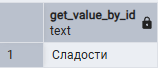
\includegraphics[width=0.25\linewidth]{img/t-6-1}
  \end{figure}
  \begin{center}
    Рисунок 12 – Результат работы функции get value by id.
  \end{center}

  \section*{Вывод}
  В ходе выполнения лабораторной работы изучены основы пользовательские функции в PostgreSQL. Созданы функции для создания или обновления данных, удаления таблицы, функция с фильтрацией данных, с использованием составного типа, триггер для логирования изменений в таблице, функцию, использующуя для получения результата динамически формируемый запрос.

\end{document}